%% Appendix
\appendix
\section{Appendix}
In this appendix, we give more precise formulations of lemmas that were mentioned in the paper, and the most important supporting definitions and lemmas.
The goal is to provide details that can help to understand in more detail what we discuss in the paper. 
Full details and proofs are not given here, but for those we refer to the technical appendix~\citep{technical_appendix}.

\subsection{Logical relation}
\label{app:logical-relation}
% Text of appendix \ldots
\textbf{$n$-subset simulation}
\begin{mathpar}
  \inferrule{(s,\phi_\pub,\phi) = (s',\phi_\pub',\phi') \\
    \forall \hat{W} \ldotp H \; (s) \; (\hat{W}) \nsubeq H' \; (s') \; (\hat{W}) }
  { (v,s,\phi_\pub,\phi,H) \nsubsim (v',s',\phi_\pub',\phi',H')}
\end{mathpar}
%
\textbf{Transition system relations}
\begin{align*}
   \Rels &= \{(\phi_\pub, \phi) \in \powerset{\States^2}\times \powerset{\States^2} \mid \phi_\pub, \phi \text{ is reflexive and transitive and } \phi_\pub \subseteq \phi \}
\end{align*}
%
\textbf{Erasure}
\begin{align*}
  \lfloor W \rfloor_S \defeq \lambda r \ldotp 
  \begin{cases}
    W(r) & W(r).v \in S\\
    \bot & \text{otherwise}
  \end{cases}
\end{align*}
%
\textbf{Active region projection}
\begin{align*}
  \activeReg{} & : \Worlds \fun 2^\RegionNames \\
  \activeReg{W} & \defeq \dom(\erase{W}{\perma,\temp})
\end{align*}
%
\textbf{Revoke temporary regions in a world}
\begin{align*}
  \revokeTemp{} & : \Worlds \fun \Worlds \\
  \revokeTemp{W} & \defeq \lambda r \ldotp 
                   \begin{cases}
                     \revoked            & \text{if }W(r) = (\temp,s,\phi_\pub,\phi,H) \\
                     W(r)                & \text{otherwise}
                   \end{cases}
\end{align*}
%
\textbf{Projection of regions based on locality}
\[
  \localityReg(\gl,W) \defeq 
  \begin{cases}
    \dom(\erase{W}{\perma ,\temp}) & \text{if } \gl = \local \\
    \dom(\erase{W}{\perma}) & \text{if } \gl = \glob
  \end{cases}
\]
%
\textbf{Address stratification}
\begin{align*}
&\iota = (v,s,\phi_\pub,\phi,H) \text{ is address-stratified iff }\\
&\qquad\begin{multlined}
  \forall s', \hat{W}, n, \ms, \ms' \ldotp \\
  \npair{\ms},\npair{\ms'} \in H~ s'~ \hat{W} \Rightarrow \\
  \dom(\ms) = \dom(\ms') \wedge \\
  \forall \addr \in
  \dom(\ms)\ldotp \npair{\ms\update{\addr}{\ms'(\addr)}} \in H~ s'~ \hat{W}
\end{multlined}
\end{align*}


\subsection{Complete ordered family of equivalences (c.o.f.e)}
\newcommand{\seq}[1]{\ensuremath{\left\{#1_n\right\}_{n=0}^{\infty}}}
\newcommand{\seqn}[1]{\ensuremath{\left(#1\right)_{n=0}^{\infty}}}
\newcommand{\NN}{\ensuremath{\mathbb{N}}}
\newcommand{\Ul}{\ensuremath{\mathcal{U}}}
\newcommand{\Later}{\ensuremath{\blacktriangleright}}
\newcommand{\op}[1]{\ensuremath{#1^{\text{op}}}}
\newcommand{\comp}{\circ}
\newcommand{\iso}{\cong}
\renewcommand{\hom}[3]{#1(#2,#3)}

\label{app:cofe}
This is an excerpt from \citet{Birkedal:tutorial-notes} about c.o.f.e.'s.
\begin{definition}[o.f.e.] An \emph{ordered family of equivalence} (o.f.e) is a
  set and a family of equivalences $\left(X, \left( \nequal \right)_{n=0}^\infty
  \right)$ that satisfy the following properties: 
  \begin{itemize}
  \item $\nequal[0]$ is the total relation on $X$
  \item $\forall n \ldotp \forall x,y \in X \ldotp x \nequal[n+1] y \Rightarrow
    x \nequal y$
  \item $\forall x,y \in X \ldotp (\forall n\ldotp x \nequal y) \Rightarrow x = y$
  \end{itemize}
  We say that an o.f.e. $\left(X, \seqn{\nequal[n]}\right)$ is \emph{inhabited} if there
  exists an element $x \in X$.
\end{definition}

If you are familiar with metric spaces observe that o.f.e.'s are but a different
presentation of bisected $1$-bounded ultrametric spaces.

\begin{definition}[Cauchy sequences and limits]
  \label{def:cauchy-sequence}
  Let $\left(X, \seqn{\nequal} \right)$ be an o.f.e. and $\seq{x}$ be a sequence of
  elements of $X$. Then $\seq{x}$ is a \emph{Cauchy sequence} if
  \begin{align*}
    \forall k \in \nats, \exists j \in \nats, \forall n \geq j, x_j \nequal[k] x_n
  \end{align*}
  or in words, the elements of the chain get arbitrarily close.

  An element $x \in X$ is the \emph{limit} of the sequence $\seq{x}$ if
  \begin{align*}
    \forall k \in \nats, \exists j \in \nats, \forall n \geq j, x \nequal[k] x_n.
  \end{align*}
  A sequence may or may not have a limit. If it has we say that the sequence
  \emph{converges}. The limit is necessarily unique in this case
  and we write $\lim_{n\to\infty}x_n$ for it.
\end{definition}

\begin{definition}[c.o.f.e.] A \emph{complete} ordered family of equivalences
  (c.o.f.e) is an o.f.e $\left(X, \left( \nequal \right)_{n=0}^\infty \right)$
  where all Cauchy sequences have a limit.  
\end{definition}

\begin{definition}
  \label{def:nonexpansive-contractive-ofe}
  Let $\left(X, \seqn{\nequal_{X}}\right)$ and $\left(Y, \seqn{\nequal_{Y}}\right)$ be
  two ordered families of equivalences and $f$ a function from the set $X$ to the set $Y$.
  The function $f$ is 
  \begin{itemize}
  \item \emph{non-expansive} if for any $x, x' \in X$, and any $n \in \nats$,
    \begin{align*}
      x \nequal_X x' \implies f(x) \nequal_Y f(x')
    \end{align*}
  \item \emph{contractive} if for any $x, x' \in X$, and any $n \in \nats$,
    \begin{align*}
      x \nequal_X x' \implies f(x) \nequal[n+1]_Y f(x')
    \end{align*}
  \end{itemize}
\end{definition}

\begin{theorem}[Banach's fixed point theorem]
  \label{thm:banach-fixed-point}
  Let $\left(X, \seqn{\nequal}\right)$ be a an inhabited c.o.f.e. and $f : X \to X$ a contractive
  function. Then $f$ has a unique fixed point.
\end{theorem}

\begin{definition}[The category $\Ul$]
  The category $\Ul$ of complete ordered families of equivalences has as objects complete
  ordered families of equivalences and as morphisms non-expansive functions.
\end{definition}

\begin{definition}
  \label{def:later-functor}
  The functor $\Later$ is a functor on $\Ul$ defined as
  \begin{align*}
    \Later\left(X, \seqn{\nequal}\right) &= \left(X,
          \seqn{\overset{n}{\equiv}}\right)\\
    \Later(f) &= f
  \end{align*}
  where $\overset{0}{\equiv}$ is the total relation and $x \overset{n+1}{\equiv} x'$
  iff $x \nequal x'$
\end{definition}

From now on, we often use the underlying set $X$ to denote a (complete) o.f.e. $\left(X,
  \seqn{\nequal}\right)$, leaving the family of equivalence
relations implicit.

\begin{definition}
 \label{def:nonexpansive-loc-contractive-functor}
 A functor $F : \op{\Ul} \times \Ul \to \Ul$ is \emph{locally non-expansive}  if for all
 objects $X$, $X'$, $Y$, and $Y'$ in $\Ul$ and
 $f, f' \in \hom{\Ul}{X}{X'}$ and $g, g' \in \hom{\Ul}{Y'}{Y}$ we have
 \begin{align*}
   f \overset{n}{=} f' \land g \overset{n}{=} g' \implies F(f, g) \overset{n}{=} F(f', g').
 \end{align*}

 It is \emph{locally contractive} if the stronger implication
 \begin{align*}
   f \overset{n}{=} f' \land g \overset{n}{=} g' \implies F(f, g) \overset{n+1}{=} F(f', g').
 \end{align*}
 holds. Note that the equalities are equalities on function spaces.
\end{definition}

\begin{proposition}
  \label{prop:loc-nonexp-loc-contr}
  If $F$ is a locally non-expansive functor then $\Later \comp F$ and $F \comp \left(\op{\Later}
  \times \Later\right)$ are locally contractive. Here, the functor $F \comp \left(\op{\Later} \times
  \Later\right)$ works as
  \begin{align*}
    (F \comp (\op{\Later} \times \Later))(X, Y) = F\left(\op{\Later}(X), \Later(Y)\right)
  \end{align*}
  on objects and analogously on morphisms and
  $\op{\Later} : \op{\Ul} \to \op{\Ul}$ is just $\Later$ working on $\op{\Ul}$ (i.e., its
  definition is the same).
\end{proposition}

\begin{definition}
 \label{def:fixed-point}
 A fixed point of a locally contractive functor $F$ is an object $X \in \Ul$, such that
 $F(X, X) \iso X$.
\end{definition}

The following is America and Rutten's fixed point theorem~\citep{America-Rutten:JCSS89}.
\begin{theorem}
 \label{thm:contr-functors-have-fixed-points}
 Every locally contractive functor $F$ such that $F(1, 1)$ is inhabited has a unique fixed
 point. The fixed point is unique among inhabited c.o.f.e.'s.
 If in addition $F(\emptyset, \emptyset)$ is inhabited then the fixed point of $F$ is unique.
\end{theorem}
In~\citet{BirkedalL:metric-enriched-journal} one can find a
category-theoretic generalization, which shows how to obtain fixed
points of locally contractive funtors on categories enriched in $\Ul$,
in particular on the category of preordered c.o.f.e.'s.  A preodered c.o.f.e. is
a c.o.f.e. equipped with a preorder that is closed under taking limits of
converging sequences.
The formulation in \emph{loc. cit.} also applies to solve
mutually recursive domain equations on preordered c.o.f.e.'s; see~\citet{bizjak:mutually-recursive-mcat}
for an explicit statement. That is the solution theorem we use to prove
Theorem~\ref{thm:world-existence}.



\subsection{Load instruction sufficiency lemma}
 \begin{lemma}[Conditions for store instruction are sufficient]
   \label{lem:conds-store-suff}
   If 
   \begin{itemize}
   \item $\ms = \ms' \uplus \ms_f$
   \item $\heapSat[\ms']{n}{W}$
   \item $((\perm,\gl),\start,\addrend,\addr) = c$
   \item $\npair{c}\in\stdvr(W)$
   \item $\writeAllowed{\perm}$
   \item $\withinBounds{\var{c}}$
   \item $\npair{\var{w}}\in\stdvr(W)$
   \item if $\var{w} = ((\_,\local),\_,\_,\_)$, then $\perm \in
     \{\rwlx,\readwritel \}$
   \end{itemize}
 
   then $\addr \in \dom(\ms')$ (i.e. $\ms\update{a}{w} =
   \ms'\update{a}{w}\uplus\ms_f$) and
   $\heapSat[{\ms'\update{\addr}{\var{w}}}]{n}{W}$
 \end{lemma}


\subsection{Macros}
\label{app:macros}
Implementation of the macros used in \texttt{scall}. Implementations of the
macros not presented here can be found in the technical
appendix~\citep{technical_appendix}.\\
\texttt{push $r$}
\begin{lstlisting}[xleftmargin=0.4cm]
  lea r_stk 1
  store r_stk r
\end{lstlisting}
\texttt{pop $r$}
\begin{lstlisting}[xleftmargin=0.4cm]
  load r r_stk
  minus r_t1 0 1
  lea r_stk r_t1
\end{lstlisting}
\texttt{rclear $r_1,\dots, r_n$}
\begin{lstlisting}[xleftmargin=0.4cm]
  move $r_1$ 0
  move $r_2$ 0
  $\dots$
  move $r_n$ 0
\end{lstlisting}
\texttt{mclear $r$}
\begin{lstlisting}[xleftmargin=0.4cm]
  move r_t $r$
  getb r_t1 r_t
  geta r_t2 r_t
  minus r_t2 r_t1 r_t2
  lea r_t r_t2
  gete r_t2
  minus r_t1 r_t2 r_t1
  plus r_t1 r_t1 1
  move r_t2 pc
  lea r_t2 $\var{off}_\var{end}$ 
  move r_t3 pc
  lea r_t3 $\var{off}_\var{iter}$
iter:
  jnz r_t2 r_t1
  store r_t 0
  lea r_t 1
  plus r_t1 r_t1 1
  jmp r_t3
end:
  move r_t 0
  move r_t1 0
  move r_t2 0
  move r_t3 0
\end{lstlisting}
Where $\var{off}_\var{end}$ and $\var{off}_\var{iter}$ are the offsets to the label \texttt{end} % 9
and \texttt{iter}, % 2
respectively.
\newline\newline
\texttt{call} $r(\bar{r}_{\var{args}},\bar{r}_{\var{priv}})$
\newline
The \texttt{call} macro constitutes a calling convention based on heap allocated activation records.
This alternative to \texttt{scall} is included to illustrate that the logical relation can be used to reason about other calling conventions.
In the following, $\bar{r}_{\var{args}}$ and $\bar{r}_{\var{priv}}$ are lists of registers. An overview of this call:
\begin{itemize}
\item Set up activation record
\item Create local enter capability for activation (protected return pointer)
\item Clear unused registers
\item Jump
\item Upon return: Run activation code
  \begin{itemize}
  \item Restore private registers
  \item Jump to return capability
  \end{itemize}
\end{itemize}
\begin{lstlisting}[xleftmargin=0.4cm]
  malloc r_t $size$ 
// store private state in activation record
  store r_t r_priv,1
  lea r_t 1
  store r_t r_priv,2
  lea r_t 1
  ...
  lea r_t 1
  store r_t r_priv,n
  lea r_t 1
// store old pc
  move r_t1 pc
  lea r_t1 $\var{off}_\var{end}$ 
  store r_t r_t1
  lea r_t1 1
// store activation record
  store r_t encode(i_1)
  lea r_t1 1
  ...
  lea r_t1 1  
  store r_t encode(i_m)
  lea r_t1 $k$ 
  restrict r_t1 encodePermPair(($\local$,e))
  move r_0 r_t1
// Clear unused registers
  rclear R // R = RegisterName - {r,pc,r_0,r_args}
  jmp r
end:
\end{lstlisting}
Where $\bar{r_{\var{priv}}} = r_{\var{priv},1}, \dots, r_{\var{priv},n}$, $size$ is the size of the activation record, $\var{off}_\var{end}$ is the offset to the \texttt{end} label, and $k$ is $m-1$, i.e. the offset to the first instruction of the activation code.\newline
The activation record. The instructions correspond to $i_1,\dots,i_m$ in the above.
\begin{lstlisting}[xleftmargin=0.4cm]
  move r_t pc
  getb r_t1 r_t
  geta r_t2 r_t
  minus r_t1 r_t1 r_t2
// load private state
  lea r_t r_t1
  load r_priv,1 r_t
  lea r_t 1
  load r_priv,2 r_t
  lea r_t 1
  ...
  lea r_t 1
  load r_priv,n r_t
  lea r_t 1
// load old pc
  load pc r_t
\end{lstlisting}

\subsection{Reasoning about programs definitions}
\label{app:programs-definitions}
\begin{definition}
  We say that $(\reg,\ms) \text{ is looking at } [i_0,\cdots,i_n] \text{ followed by } c_{\mathit{next}}$ 
  iff
  \begin{itemize}
  \item $\reg(\pcreg) = ((p,g),b,e,a)$
  \item $p = \rwx$, $p = \exec$, or $p = \rwlx$
  \item $a+n\leq e$, $b\leq a\leq e$
  \item $\ms(a+0,\cdots,a+n) = [i_0,\cdots,i_n]$
  \item $c_{\mathit{next}} = ((p,g),b,e,a+n+1)$
  \end{itemize}
\end{definition}

\begin{definition}
  We say that ``\linksto{(\reg,\ms)}{\var{key}}{j}{c}'' 
  iff
  \begin{itemize}
  \item $\reg(pc) = \stdcap$
  \item $\ms(\start) = ((\_,\_),\start_\link,\_,\_)$
  \item $\ms(\start_\link+j) = c$
  \end{itemize}
\end{definition}

\begin{definition}
  We say that $\reg \text{ points to stack with $\ms_\stk$ used and $\ms_{\mathit{unused}}$ unused}$
  iff
  \begin{itemize}
  \item $\reg(r_\stk) =((\rwlx,\local),b_\stk,e_\stk,a_\stk)$
  \item $\dom(\ms_{\mathit{unused}}) = [a_\stk+1,\cdots,e_\stk]$
  \item $\dom(\ms_\stk) = [b_\stk,\cdots,a_\stk]$ \lau{Maybe make it clear what happens when $\ms_\stk$ is empty}
  \item $b_\stk - 1\leq a_\stk$
  \end{itemize}
\end{definition}


 \subsection{Example correctness lemmas}
\begin{lemma}[Correctness lemma for \texttt{f1}, copy of Lemma~\ref{lem:correctness-f1}] \forcenewline
  \label{lem:correctness-f1-app}
  For all $n \in \nats$
  let
  \begin{align*}
    c_{\var{adv}} & \defeq ((\entry,\glob),\start_{\adv},\addrend_{\adv},\start_{\adv}+\olf) \\
    c_{f1} & \defeq ((\rwx,\glob),\mathtt{f1}-\olf,\mathtt{1f},\mathtt{f1}) \\
    c_\malloc & \defeq ((\entry,\glob),\start_\malloc,\addrend_\malloc,\start_\malloc+\olf) \\
    m & \defeq \hs_{f1} \uplus 
        \hs_\flag \uplus                
        \ms_{\var{link}} \uplus 
        \hs_\adv \uplus 
        \ms_{\malloc} \uplus 
        \hs_{\var{frame}} 
  \end{align*}
  and
  \begin{itemize}
  \item $c_\malloc$ satisfies the specification for malloc and $\iota_{\malloc,0}$ is the region from the specification.
  \end{itemize}
  where 
  \begin{align*}
    &\dom(\hs_{f1}) = [\mathtt{f1}-\olf,\mathtt{1f}] \\
    &\dom(\hs_\flag) = [\flag,\flag] \\
    &\dom(\ms_\link) = [\link,\link+1]\\
    &\dom(\hs_{\adv}) = [\start_\adv,\addrend_\adv] \\
    &\heapSat[\hs_{\malloc}]{n}{[0 \mapsto \iota_{\malloc,0}]}
  \end{align*}
  and
  \begin{itemize}
  \item $\ms_{f1}(\mathtt{f1}-\olf) = ((\readonly,\glob),\link,\link+1,\link)$, $\ms_{f1}(\mathtt{f1}-\olf+1) = ((\readwrite,\glob),\flag,\flag,\flag)$, the rest of $\hs_{f1}$ contains the code of $f1$.
  \item $\ms_\flag = [\flag \mapsto 0]$
  \item $\ms_{\var{link}} = [\var{link} \mapsto c_\malloc, \var{link} + 1 \mapsto c_\adv]$
  \item $\hs_\adv$ contains a global read-only capability for $\hs_\link$ on its first address. The remaining cells of the memory segment only contain instructions.
  \end{itemize}
  if 
  \[
    (\reg\update{\pcreg}{c_{f1}},m) \step[n] (\halted,m'),
  \]
  then
  \[
    m'(\flag) = 0
  \]  
\end{lemma}

\begin{lemma}[Correctness lemma for \texttt{f2}, detailed version of Lemma~\ref{lem:correctness-f2}]
  \label{lem:correctness-f2-app}
  let
  \begin{align*}
    c_{\var{adv}} & \defeq ((\entry,\glob),\start_{\adv},\addrend_{\adv},\start_{\adv}+\olf) \\
    c_{f2} & \defeq ((\rwx,\glob),\mathtt{f2}-\olf,\mathtt{2f},\mathtt{f2}) \\
    c_\malloc & \defeq ((\entry,\glob),\start_\malloc,\addrend_\malloc,\start_\malloc+\olf) \\
    c_{\var{stk}} & \defeq ((\rwlx,\local),\start_\stk,\addrend_\stk,\start_\stk-1) \\
    c_\link & \defeq ((\readonly,\glob),\link,\link+1,\link)\\
    \reg & \in \Regs \\
    m & \defeq \hs_{f2} \uplus 
        \hs_\flag \uplus                
        \ms_{\var{link}} \uplus 
        \hs_\adv \uplus 
        \ms_{\malloc} \uplus 
        \ms_{\var{stk}} \uplus
        \ms_{\var{frame}} 
  \end{align*}
  and
  \begin{itemize}
  \item $c_\malloc$ satisfies the specification for malloc and $\iota_{\malloc,0}$ is the region from the specification.
  \end{itemize}
  where 
  \begin{align*}
    &\dom(\hs_{f2}) = [\mathtt{f2}-\olf,\mathtt{2f}] \\
    &\dom(\hs_\flag) = [\flag,\flag] \\
    &\dom(\ms_\link) = [\link,\link+1]\\
    &\dom(\ms_\stk) = [\start_\stk, \addrend_\stk]\\
    &\dom(\hs_{\adv}) = [\start_\adv,\addrend_\adv] \\
    &\heapSat[\hs_{\malloc}]{n}{[0 \mapsto \iota_{\malloc,0}]} \qquad \text{ for all $n \in \nats$}
  \end{align*}
  and
  \begin{itemize}
  \item $\ms_{f2}(\mathtt{f2}-\olf) = ((\readonly,\glob),\link,\link+1,\link)$, $\ms_{f2}(\mathtt{f2}-\olf+1) = ((\readwrite,\glob),\flag,\flag,\flag)$, the rest of $\hs_{f2}$ contains the code of $f2$.
  \item $\ms_\flag = [\flag \mapsto 0]$
  \item $\ms_{\var{link}} = [\var{link} \mapsto c_\malloc, \var{link} + 1 \mapsto c_\adv]$
  \item $\hs_\adv(\start_\adv) = c_\link$ and $\forall \addr \in [\start_\adv+1,\addrend]\ldotp \ms_\adv(a) \in \ints$
  \end{itemize}
  if 
  \[
    (\reg\update{\pcreg}{c_{f2}}\update{r_\stk}{c_\stk},m) \step[n] (\halted,m'),
  \]
  then
  \[
    m'(\flag) = 0
  \]  
\end{lemma}
\begin{lemma}[Correctness lemma for \texttt{f3}, detailed version of Lemma~\ref{lem:correctness-f3}]
  \label{lem:correctness-f3-detailed}
  For all $n \in \nats$
  let
  \begin{align*}
    c_{\var{adv}} & \defeq ((\entry,\glob),\start_{\adv},\addrend_{\adv},\start_{\adv}+\olf) \\
    c_{f3} & \defeq ((\rwx,\glob),\mathtt{f3}-\olf,\mathtt{3f},\mathtt{f3}) \\
    c_{\var{stk}} & \defeq ((\rwlx,\local),\start_\stk,\addrend_\stk,\start_\stk-1) \\
    c_\malloc & \defeq ((\entry,\glob),\start_\malloc,\addrend_\malloc,\start_\malloc+\olf) \\
    c_\link & \defeq ((\readonly,\glob),\link,\link+1,\link) \\
    \reg & \in \Regs \\
    m & \defeq \hs_{f3} \uplus 
        \hs_\flag \uplus                
        \ms_{\var{link}} \uplus 
        \hs_\adv \uplus 
        \ms_{\malloc} \uplus 
        \ms_{\var{stk}} \uplus
        \ms_{\var{frame}} 
  \end{align*}
  and
  \begin{itemize}
  \item $c_\malloc$ satisfies the specification for malloc.
  \end{itemize}
  where 
  \begin{align*}
    &\dom(\hs_{f3}) = [\mathtt{f3}-\olf,\mathtt{3f}] \\
    &\dom(\hs_\flag) = [\flag,\flag] \\
    &\dom(\ms_\link) = [\link,\link+1]\\
    &\dom(\ms_\stk) = [\start_\stk, \addrend_\stk]\\
    &\dom(\hs_{\adv}) = [\start_\adv,\addrend_\adv] \\
    &\heapSat[\hs_{\malloc}]{n}{[0 \mapsto \iota_{\malloc,0}]}
  \end{align*}
  and
  \begin{itemize}
  \item $\ms_{f3}(\mathtt{f3}-\olf) = ((\readonly,\glob),\link,\link+1,\link)$, $\ms_{f3}(\mathtt{f3}-\olf+1) = ((\readwrite,\glob),\flag,\flag,\flag)$, the rest of $\hs_{f3}$ contains the code of $f3$.
  \item $\ms_\flag = [\flag \mapsto 0]$
  \item $\ms_{\var{link}} = [\var{link} \mapsto c_\malloc, \var{link} + 1 \mapsto c_\adv]$
  \item $\hs_\adv(\start_\adv) = c_\link$ and all other addresses of $\ms_\adv$ contain instructions.
  \end{itemize}
  if 
  \[
    (\reg\update{\pcreg}{c_{f3}}\update{r_\stk}{c_\stk},m) \step[n] (\halted,m'),
  \]
  then
  \[
    m'(\flag) = 0
  \]  
\end{lemma}

 
 \begin{lemma}[Correctness of $g1$, detailed version of Lemma~\ref{lem:correctness-g1}]
  \label{lem:correctness-g1-detailed}
  For all $n \in \nats$
  let
  \begin{align*}
    c_{\var{adv}} & \defeq ((\rwx,\glob),\start_{\adv},\addrend_{\adv},\start_{\adv}+\olf) \\
    c_{g1} & \defeq ((\entry,\glob),\mathtt{g1}-\olf,\mathtt{4f},\mathtt{g1}) \\
    c_\stk & \defeq ((\rwlx,\local),\start_\stk,\addrend_\stk,\start_\stk-1) \\
    c_\malloc & \defeq ((\entry,\glob),\start_\malloc,\addrend_\malloc,\start_\malloc+\olf) \\
    c_\link & \defeq ((\readonly,\glob),\link,\link,\link) \\
    m & \defeq \hs_{g1} \uplus 
        \ms_\flag \uplus                
        \ms_\link \uplus 
        \ms_\adv \uplus 
        \ms_\malloc \uplus 
        \ms_\stk \uplus
        \ms_{\var{frame}} 
  \end{align*}
  where 
  \begin{itemize}
  \item $c_\malloc$ satisfies the specification for malloc with $\iota_{\malloc,0}$
  \end{itemize}
  \begin{align*}
    &\dom(\hs_{g1}) = [\mathtt{g1}-\olf,\mathtt{4f}] \\
    &\dom(\hs_\flag) = [\flag,\flag] \\
    &\dom(\ms_\link) = [\link,\link]\\
    &\dom(\ms_\stk) = [\start_\stk, \addrend_\stk]\\
    &\dom(\hs_{\adv}) = [\start_\adv,\addrend_\adv] \\
    &\heapSat[\hs_{\malloc}]{n}{[0 \mapsto \iota_{\malloc,0}]}
  \end{align*}
  and
  \begin{itemize}
  \item $\ms_{g1}(\mathtt{g1}-\olf) = ((\readonly,\glob),\link,\link,\link)$, $\ms_{g1}(\mathtt{g1}-\olf+1) = ((\readwrite,\glob),\flag,\flag,\flag)$, the rest of $\hs_{g1}$ contains the code of $g1$ immediately followed by the code of $f4$.
  \item $\ms_\flag = [\flag \mapsto 0]$
  \item $\ms_{\var{link}} = [\link \mapsto c_\malloc]$
  \item $\hs_\adv(\start_\adv) = c_\link$ and all other addresses of $\ms_\adv$ contain instructions.
  \item $\forall a \in \dom(\ms_\stk) \ldotp \ms_\stk(a) = 0$ %This condition could be weakened to \memSat{\ms_\stk}{[\iota^\pwl(\dom(\ms_\stk))]}
  \end{itemize}
  if 
  \[
    (\reg_0\update{\pcreg}{c_\adv}\update{r_\stk}{c_\stk}\update{r_1}{c_{g1}},m) \step[n] (\halted,m'),
  \]
  then
  \[
    m'(\flag) = 0
  \]  
\end{lemma}


\subsection{Awkward example}
\label{app:awkward-example}
\textbf{The region for variable $x$} The region $\iota_x$, is the region omitted from the proof sketch for the awkward example.
\figurename~\ref{fig:x-reg} illustrates the transition system of $\iota_x$.
  \begin{figure}[tb]
    \centering
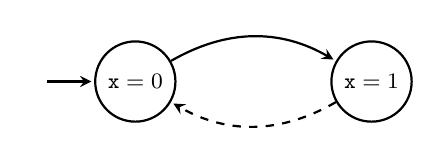
\begin{tikzpicture}[->,shorten >=1pt,auto,node distance=3cm,
  thick,main node/.style={circle,fill=white,draw,font=\sffamily\large},rect node/.style={rectangle,fill=blue!20,draw,font=\sffamily\large}]

  \node[main node] (n0) {\footnotesize $\texttt{x}=0$};
  \node (s) [left of=n0,xshift=1.75cm] {  };
  \node[main node] (n1) [right of=n0]  {\footnotesize $\texttt{x}=1$};
  \draw (s) edge[>=stealth] (n0);
  \draw (n0) edge[bend left,>=stealth] (n1);
  \draw (n1) edge[bend left,dashed,>=stealth] (n0);
  
\end{tikzpicture}
  \caption{Illustration of transition system in $\iota_x$. The dashed line is
    the private transition.}
  \label{fig:x-reg}
\end{figure}

\begin{definition}
  \label{def:iotax-region}
  \begin{align*}
    \iota_x   & = (\perm, 0, \phi_\pub, \phi, H_x) \\
    \phi_\pub & = \{(0,1)\}^* \\
    \phi      & = (1,0) \union \phi_\pub \\
    H_x \; s \; \hat{W} & = \{\npair{\ms} \mid \ms(x) = s \land n > 0 \} \union \{\npair[0]{\ms}\}
  \end{align*}
\end{definition}
\textbf{Static region} This static region only requires that the memory segment is the given one.
As it does not require safety, capabilities for this region cannot be gives to adversarial code.
\begin{align*}
  \iota^\sta (v,\ms) &= (v,1,=,=,H^\sta\;\ms)\\
  H^\sta \; \ms \; s \; \hat{W} = & \{\npair{\ms} \mid n > 0 \} \union \{\npair[0]{\ms'} \mid \ms' \in \Mems \}
\end{align*}
\textbf{Static safe region} Static region that also requires safety.
It is safe to give adversarial code read capabilities for this region.
\begin{align*}
  \iota^{\sta,u} (v,\ms) &= (v,1,=,=,H^{\sta,u}\;\ms)\\
  H^{\sta,u} \; \ms \; s \; \hat{W} = & \left\{\npair{\ms'} \middle|
    \begin{aligned}
      &\ms' = \ms \land{}\\
      &\forall \addr \in \dom(\ms) \ldotp\\
      & \quad \nonlocal{\ms(\addr)} \land{}\\
      & \quad \npair[n-1]{\ms(\addr)} \in \stdvr(\xi(\hat{W}))
    \end{aligned}
        \right\} \union \{\npair[0]{\ms'} \mid \ms' \in \Mems \}
\end{align*}


